%http://cs.pugetsound.edu/~jross/courses/cs240/project/requirements/
%Animation Group
\documentclass[12pt]{article}
\usepackage{graphicx}
\begin{document}

<<<<<<< HEAD
=======



>>>>>>> master
% Front Page
\begin{titlepage}
	\begin{center}
	\huge  Edith \\
	\vspace*{\fill}%
 	\huge \textsc{\textbf{Animation Team \\Requirement Specifications} }	
	\bigskip 
	\rule{130mm}{.1pt}
<<<<<<< HEAD
	\textsc{\textbf{September 25, 2013 \\ Revised: October 2, 2013} \\ }	
=======
	\textsc{\textbf{September 25, 2013 \\ Revised: September 28, 2013} \\ }	
>>>>>>> master
	\vspace*{\fill}%
	Eric Lund \\
	Kramer Canfield \\ 
	Zeke Rosenberg \\
	Calder Whiteley \\
	Jon Youmans
	\end{center}
	\end{titlepage}

% Next page

%Executive Summary
\section{\emph{Executive Summary}}
<<<<<<< HEAD
One of the components of the "Edith" system, a 2D web-based computer science teaching tool, is the Animation System. The Animation System module is important because it includes the core animation frameworks and specifications of how the animations and audio will be produced. In a visually-based programming environment, this module is clearly important because it provides animations without requiring the user to have any knowledge of a scripting language or computer graphics concepts. There are two use cases for this module: creating new media and navigating existing media. The media is specified by a different sub-system which delivers the instructions to the Animation System module. The Animation System processes the instructions (assuming the instructions are delivered correctly) and delivers the animations to another sub-system to be displayed on the screen as desired.
=======
One of the components of the "Edith" system, a 2D web-based computer science teaching tool, is the Animation System module, a sub-system of Edith. The Animation System module is important because it includes the core animation frameworks and specifications of how the animations and audio will be produced. In a visually-based programming environment, this module is clearly important because it provides animations without requiring the user to have any knowledge of a scripting language or computer graphics concepts. There is only one use case for this module: provide animations and play sounds. The animations are specified by a different sub-system which delivers the instructions to the Animation System module. The Animation System processes the instructions (assuming the instructions were delivered correctly) and delivers the animations and audio to another sub-system to be displayed on the screen as desired.
>>>>>>> master


%Introduction
\section{\emph{Introduction}}%Create a section for the introduction
	\subsection{Edith}
<<<<<<< HEAD
         Edith is a 2D, web-based system used to help students learn to program and get excited about computer science. The system will allow students to program relationships among objects in a virtual world in order to create animations. It will offer several useful capabilities: users will be able to create objects for their story using a graphical, drag and drop interface; specify animated behaviors for these objects using a visual programming language; add user interactions to create game-like experiences; and share their creations with others. 
	\subsection{Module}
	The Animation Module accepts a properly formatted instruction set to construct an animated scene. An animated scene consists of a canvas that can include pre-defined image sprites and pre-defined audio files provided by the Object Creator Module. The scene is installed in the final UI by the Story Creator Module. Playback of the media is also handled by the Animation System.
	\subsection{Purpose}
        The Animation Module allows the user to render animations without knowledge of a scripting language. This is possible by applying pre-defined animation sets to image sprites. The module also allows the user to include audio with their animations. The module is intended to interpret animation instructions and render an animation sequence.

% Use Cases
\section{\emph{Functional Requirements}}
	\subsection{``Use Case 1: Create Media"}
\begin{enumerate}
  \item Actor
  \begin{enumerate}
  		\item ``Drawer": The Edith sub-system providing us with sprites to animate and a list of media creation instructions.
   		 \item ``Taker": The Edith sub-system that takes and displays our media.
       \item ``Programmer": The individual who is using Edith through his/her web browser to learn how to program.
  \end{enumerate}
  \item Preconditions/Assumptions
  \begin{enumerate}
   		 \item Preconditions: The ``Programmer" has already defined which sprites will be animated.
=======
         Edith is a 2D, web-based system to help students learn to program and get excited about computer science. The system will allow students to program relationships among objects in a virtual world, in order to create animations. It will offer several useful capabilities: users will be able to create objects for their story using a graphical, drag and drop interface; specify animated behaviors for these objects using a visual programming language; add user interactions to create game-like experiences; and share their creations with others. 
	\subsection{Module}
	The Animation Module accepts a properly formatted instruction set to construct an animated scene. An animated scene consists of a canvas that can include pre-defined image sprites and pre-defined audio files provided by the Object Creator Module. The scene is installed in the final UI by the Story Creator Module. 
	\subsection{Purpose}
        The Animation Module allows the user to render animations without knowledge of a scripting language. This is possible by applying pre-defined animation sets to image sprites. The module also allows the user to include audio with their animations. The module is intended to interpret animation instructions and render an animation sequence.


% Use Cases
\section{\emph{Functional Requirements}}
	\subsection{"Use Case 1: Providing Animations and Playing Sounds"}
\begin{enumerate}
  \item Actor
  \begin{enumerate}
  		\item "Drawer": The system providing us with sprites to animate and sounds to play.
   		 \item "Taker": The system that takes and displays our canvas.
		\item Animation System: The system we are creating that handles back-end animation and final.
  \end{enumerate}
  \item Preconditions/Assumptions
  \begin{enumerate}
   		 \item Preconditions: The user has already defined which sprites will be animated and which sounds will be played.
>>>>>>> master
   		 \item Assumptions: The web browser supports HTML5 and JavaScript.
  \end{enumerate}
  \item Flow of Events
  \begin{enumerate}
<<<<<<< HEAD
   		 \item The ``Drawer" provides media creation instructions to the Animation System. (The instructions must follow the Animation System's specification.)
   		 \item The Animation System processes the instructions and pulls out the relevant data such as the sprite or image to draw, the animation method (e.g. rotate, move, etc.), parameters of the method, and associated sound files.
		\item The Animation System creates media in a frame-based format. In other words, for each frame,the animations provided are a sequence of drawing commands for the canvas. The effect of viewing many frames of drawing commands will be the same as watching a traditional format of video or film.
		\item The Animation System provides the drawing commands to the ``Taker" for final display on the canvas and at the same time plays the associated audio file(s), given in a standard digital-audio format such as .wav, .mp3, or another standard.
  \end{enumerate}
  \item Alternatives
  \begin{enumerate}
    		\item The ``Drawer" provides faulty input, discovered during vaildation of the instructions.
		    \item The Animation System asks for good input from the ``Drawer" until good input is provided, then the flow of events above is followed through completion.
  \end{enumerate}
  %\item  Postconditions
  %\begin{enumerate}
  % 		\item
  %\end{enumerate}
\end{enumerate}



  \subsection{``Use Case 2: Navigate Existing Media"}
\begin{enumerate}
  \item Actor
  \begin{enumerate}
      \item ``Drawer": The Edith sub-system providing us with sprites to animate and a list of media creation instructions.
       \item ``Taker": The Edith sub-system that takes and displays our media.
       \item ``Programmer": The individual who is using Edith through his/her web browser to learn how to program.
  \end{enumerate}
  \item Preconditions/Assumptions
  \begin{enumerate}
       \item Preconditions: The "Programmer" has already defined which sprites will be animated and which sounds will be played.
       \item Assumptions: The web browser supports HTML5 and JavaScript.
       \item A User interface for playback controls has been created and is ready to use by the ``Programmer."
  \end{enumerate}
  \item Flow of Events
  \begin{enumerate}
      \item The ``Drawer" calls one of the playback control functions provided by the Animation System: play, pause, or seek. Additional playback controls may be added. Note: The seek function is not the same as scrubbing through a video; the ``Programmer" will enter or select a time location in the animations and the media will play from that selected time.
      \item The Animation System determines which frame(s) needs to be drawn based on the function called and gives that frame to the ``Taker" for final display. For instance, if the media is paused, the animations will stop and any associated audio will not be played.
  \end{enumerate}
  \item Alternatives
  \begin{enumerate}
        \item No alternative flow-of-events. Invalid input from the ``Programmer" should be handled by the ``Drawer."
  \end{enumerate}
  %\item  Postconditions
  %\begin{enumerate}
  %     \item
  %\end{enumerate}
\end{enumerate}
	
\subsection{Activity Diagram}
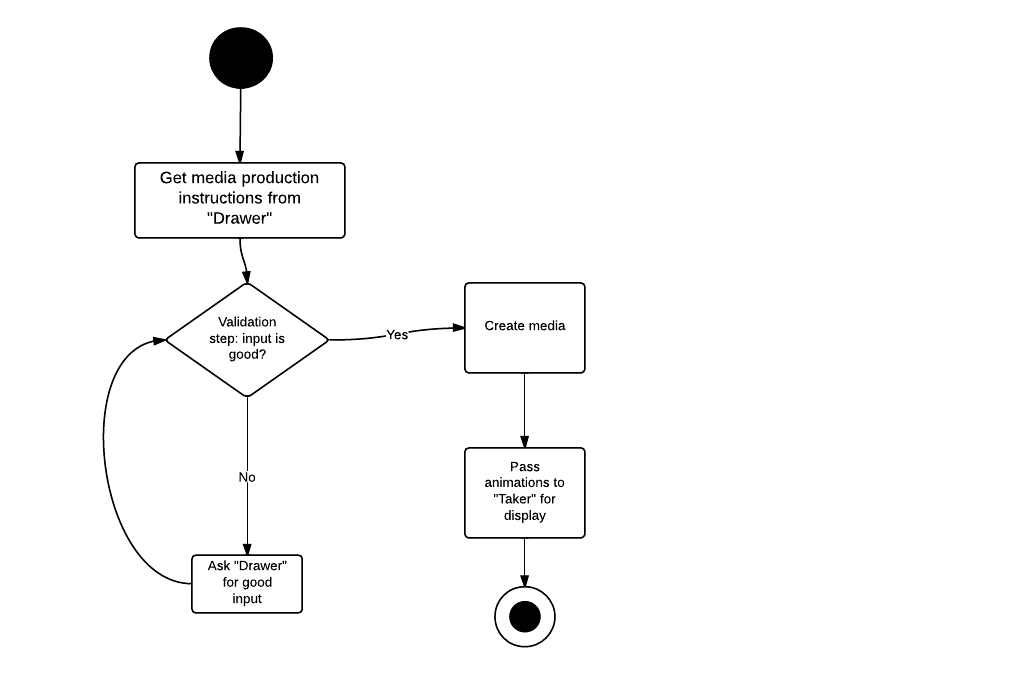
\includegraphics[scale=.45]{Activity_Diagram.png}
\\Activity Diagram of Use Case 1
=======
   		 \item "Drawer" provides drawing instructions to the Animation System. 
   		 \item The Animation System processes the instructions.
		\item The Animation System creates animations and plays sounds.
		\item The Animation System provides the animations to the "Taker."
  \end{enumerate}
  \item Alternatives
  \begin{enumerate}
    		\item The "Drawer" provides faulty drawing instructions.
    		\item The Animation System attempts and fails to process instructions.
		\item The Animation System passes the error to the "Taker."
  \end{enumerate}
  %\item  Postconditions
  %\begin{enumerate}
  % 		\item 
  %\end{enumerate}
\end{enumerate}

	

\subsection{UML}
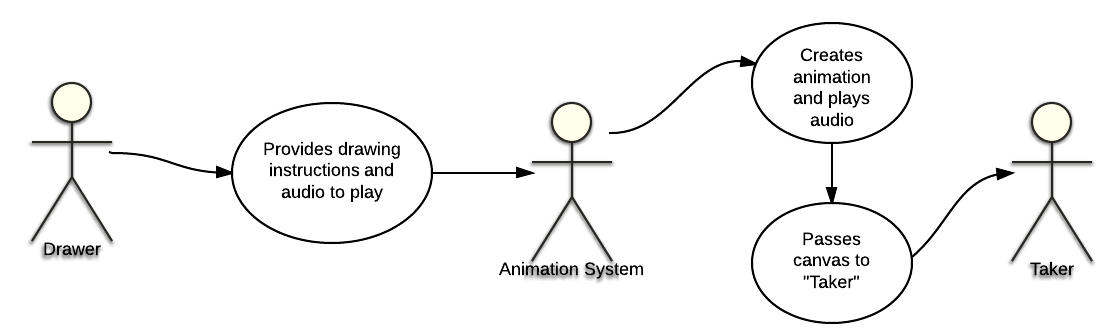
\includegraphics[scale=.4]{UML.png}
UML Diagram of Animation System Flow of Events
>>>>>>> master


%Nonfunctional Requirements
\section{\emph{Nonfunctional Requirements}}

\begin{itemize}
	\item Ease-of-Use: Specific documentation of options for animation provided to the "Drawer" on animations that we can provide.
	\item Documentation: Specific documentation of instructions provided to the "Taker" on how to receive the dynamic picture frame (the canvas).
\end{itemize}

%Glossary/References
\section{\emph{Glossary/References}}
Glossary:
\begin{itemize}
	\item Canvas: The JavaScript and HTML5 "dynamic picture frame" to give to the "Taker."
<<<<<<< HEAD
	\item Sprite:  a computer graphic that may be moved on-screen and otherwise manipulated as a single entity (New Oxford American Dictionary (American English))
=======
	\item Sprite:  a computer graphic that may be moved on-screen and otherwise manipulated as a single entity
>>>>>>> master
\end{itemize}

\noindent References: 
\begin{itemize}
<<<<<<< HEAD
=======
	\item LaTeX WikiBook http://en.wikibooks.org/wiki/LaTeX
>>>>>>> master
	\item Edith Project Description http://cs.pugetsound.edu/~jross/courses/cs240/project/edith/
	\item New Oxford American Dictionary (American English)
\end{itemize}

\end{document}
